% !TeX spellcheck = en_US
\documentclass[12pt]{article}
\usepackage[a4paper, margin=1.25in]{geometry}
\usepackage[utf8]{inputenc}
\usepackage{amsmath}
\usepackage{amsfonts}
\usepackage{amssymb}
\usepackage{graphicx}
\usepackage{mathtools}
\usepackage[pageanchor, hidelinks]{hyperref}  % most people dont know of this :3

\usepackage{float}
\usepackage{xfrac}


\usepackage{booktabs}
\usepackage{tabularx}

%\usepackage{subfig}
\usepackage{subcaption}
% \usepackage[margin=0.7in]{geometry}

\usepackage[backend=bibtex,style=verbose-ibid]{biblatex}
\addbibresource{citations.bib}

\usepackage{listings}
\usepackage{color}
\definecolor{dkgreen}{rgb}{0,0.6,0}
\definecolor{gray}{rgb}{0.5,0.5,0.5}
\definecolor{mauve}{rgb}{0.58,0,0.82}

\lstset{frame=tb,
  language=Python,
  aboveskip=3mm,
  belowskip=3mm,
  showstringspaces=false,
  columns=flexible,
  basicstyle={\small\ttfamily},
  numbers=none,
  numberstyle=\tiny\color{gray},
  keywordstyle=\color{blue},
  commentstyle=\color{dkgreen},
  stringstyle=\color{mauve},
  breaklines=true,
  breakatwhitespace=true,
  tabsize=3
}

\providecommand{\main}{..} 
\graphicspath{{\main/images/}{images/}}


\usepackage{pdfpages}

\usepackage[english]{babel}
\usepackage[autostyle, english = american]{csquotes}
\MakeOuterQuote{"}

\author{jcn514}
\title{IB Music Presenting}
\date{April 15th, 2023}

\begin{document}
\maketitle
\tableofcontents

\pagebreak


\section{Presenting as a Creator}


\subsection{"Zenith" An Orchestral Composition (AOI 2)}

Inspired by orchestral music in video games, I composed \textit{Zenith} as an exercise to learn the capabilities of individual instruments and the resulting effects of their combination. I intended to emulate the grand texture and movement of franchises like Super Mario Galaxy, Octopath Traveler and Hollow Knight. This falls under AOI 2 because it was composed primarily for listening and enjoyment. Using the notation software Musescore 4, I brainstormed with my primary instrument, the piano, and used knowledge to arrange parts for the orchestra. This piece emphasizes texture and motivic development through harmonization, call and response, and voice leading throughout its instrumentation.


\hyperlink{page.5}{\textit{The sheet music is the first attachment in the appendix.}}

\subsection{"Constellations" A Choral Piece; 5th Graders (AOI 1)}

For our inter-school global concert, I sought to compose an original choral piece for our 5th grade choir. I composed the instrumental with melody, collaboration with my elementary school music teacher and the 5th graders on the lyrics. The piece, Constellations, centers on empowering kids to take action in finding their passion and having a positive impact on the world around them—in line with the concert’s theme of global community—falling under AOI 1. I aimed for simplicity in the harmony which would be nicely complemented by tactful voicings and implied chord extensions.

\hyperlink{page.22}{\textit{The sheet music is the second attachment in the appendix.}}

\section{Presenting as a Performer}

\subsection{"Secret of the Forest"—Y. Mitsuda (AOI 4)}

I performed Japanese composer Yasunori Mitsuda’s acclaimed electronic song, \textit{Secret of the Forest}. I chose this song because of Mitsuda’s strong melodic focus and innovative use of mode mixture and unorthodox harmony. He combines these musical elements within the expressiveness of the late 90’s electronic music trends—falling under AOI 4. In my arrangement, I referenced a number of existing piano reductions to combine the most important voices and features of each section to preserve MItsuda’s artistic intent. For instance, I enjoyed Zohair002’s middle section with the modified right hand arpeggios, opting to do something similar in my own arrangement.\autocite{youtube}


\subsection{"Jeux d'eau"—M. Ravel (AOI 2)}

I performed my own rendition of Maurice Ravel’s (1835–1937) early composition, \textit{Jeux d’Eau}, which loosely translates to fountains or water games. First performed in 1902, this piece was deemed ‘unmusical’ by Ravel’s teachers, since it forwent the classical tonality in favor of emulating the noise and musical sounds of cascading, spraying water. Although Ravel rejected the term, this piece falls into the genre of Impressionism. The striking elements of this piece include its delicate, yet layered musical texture, which doesn't shy away from dissonance when appropriate. When you listen, focus on my interpretation of water through the slurs of quick, quiet notes.

\subsection{Ocarina of Time Piano Medley—E. Correll (AOI 3)}

My last performance paid homage to my enjoyment of the videogame music genre and the Zelda franchise. I learnt and performed Erik Corell’s Piano Medley, based on Koji Kondo music for The Legend of Zelda: Ocarina of Time.\autocite{zelda} This highly-technical arrangement includes many well-known Zelda songs, like The \textit{Song of Storms}, \textit{Great Fairy’s Fountain}, \textit{Gerudo Valley}, and \textit{The Lost Woods}, while adding a virtuoso flair to many sections. I enjoyed challenging myself technically with this piece because it also demanded me to explore new styles on the piano. However, the difficulty of the piece became an obstacle to performing it confidently, so it demanded many hours of practice to improve minor sections—inspiring new discipline into the way I approach music.

\section{Track List}

\begin{table}[H]
\centering
\begin{tabularx}{0.9\textwidth}{@{}lX@{}X@{}}
\toprule
\textbf{Track} & \textbf{Start} & \textbf{End} \\ \midrule
"Zenith" An Orchestral Composition & 0:00 & 3:27 \\
"Constellations" A Choral Piece w/ 5th Graders & 3:38 & 6:28 \\ \bottomrule
\end{tabularx}
\caption{Presenting as a Creator}
\vspace*{0.5cm}
\begin{tabularx}{0.9\textwidth}{@{}lX@{}X@{}}
\toprule
\textbf{Track} & \textbf{Start} & \textbf{End} \\ \midrule
"Secret of the Forest"—Y. Mitsuda (Arr. me) & 6:32 & 8:54 \\
"Jeux d'eau"—M. Ravel & 9:03 & 14:22 \\
Zelda Ocarina of Time Piano Medley—E. Correll & 14:26 & 18:38 \\ \bottomrule
\end{tabularx}
\caption{Presenting as a Performer}
\end{table}


\section{References}
\printbibliography[heading=none]

\section{Music Scores}
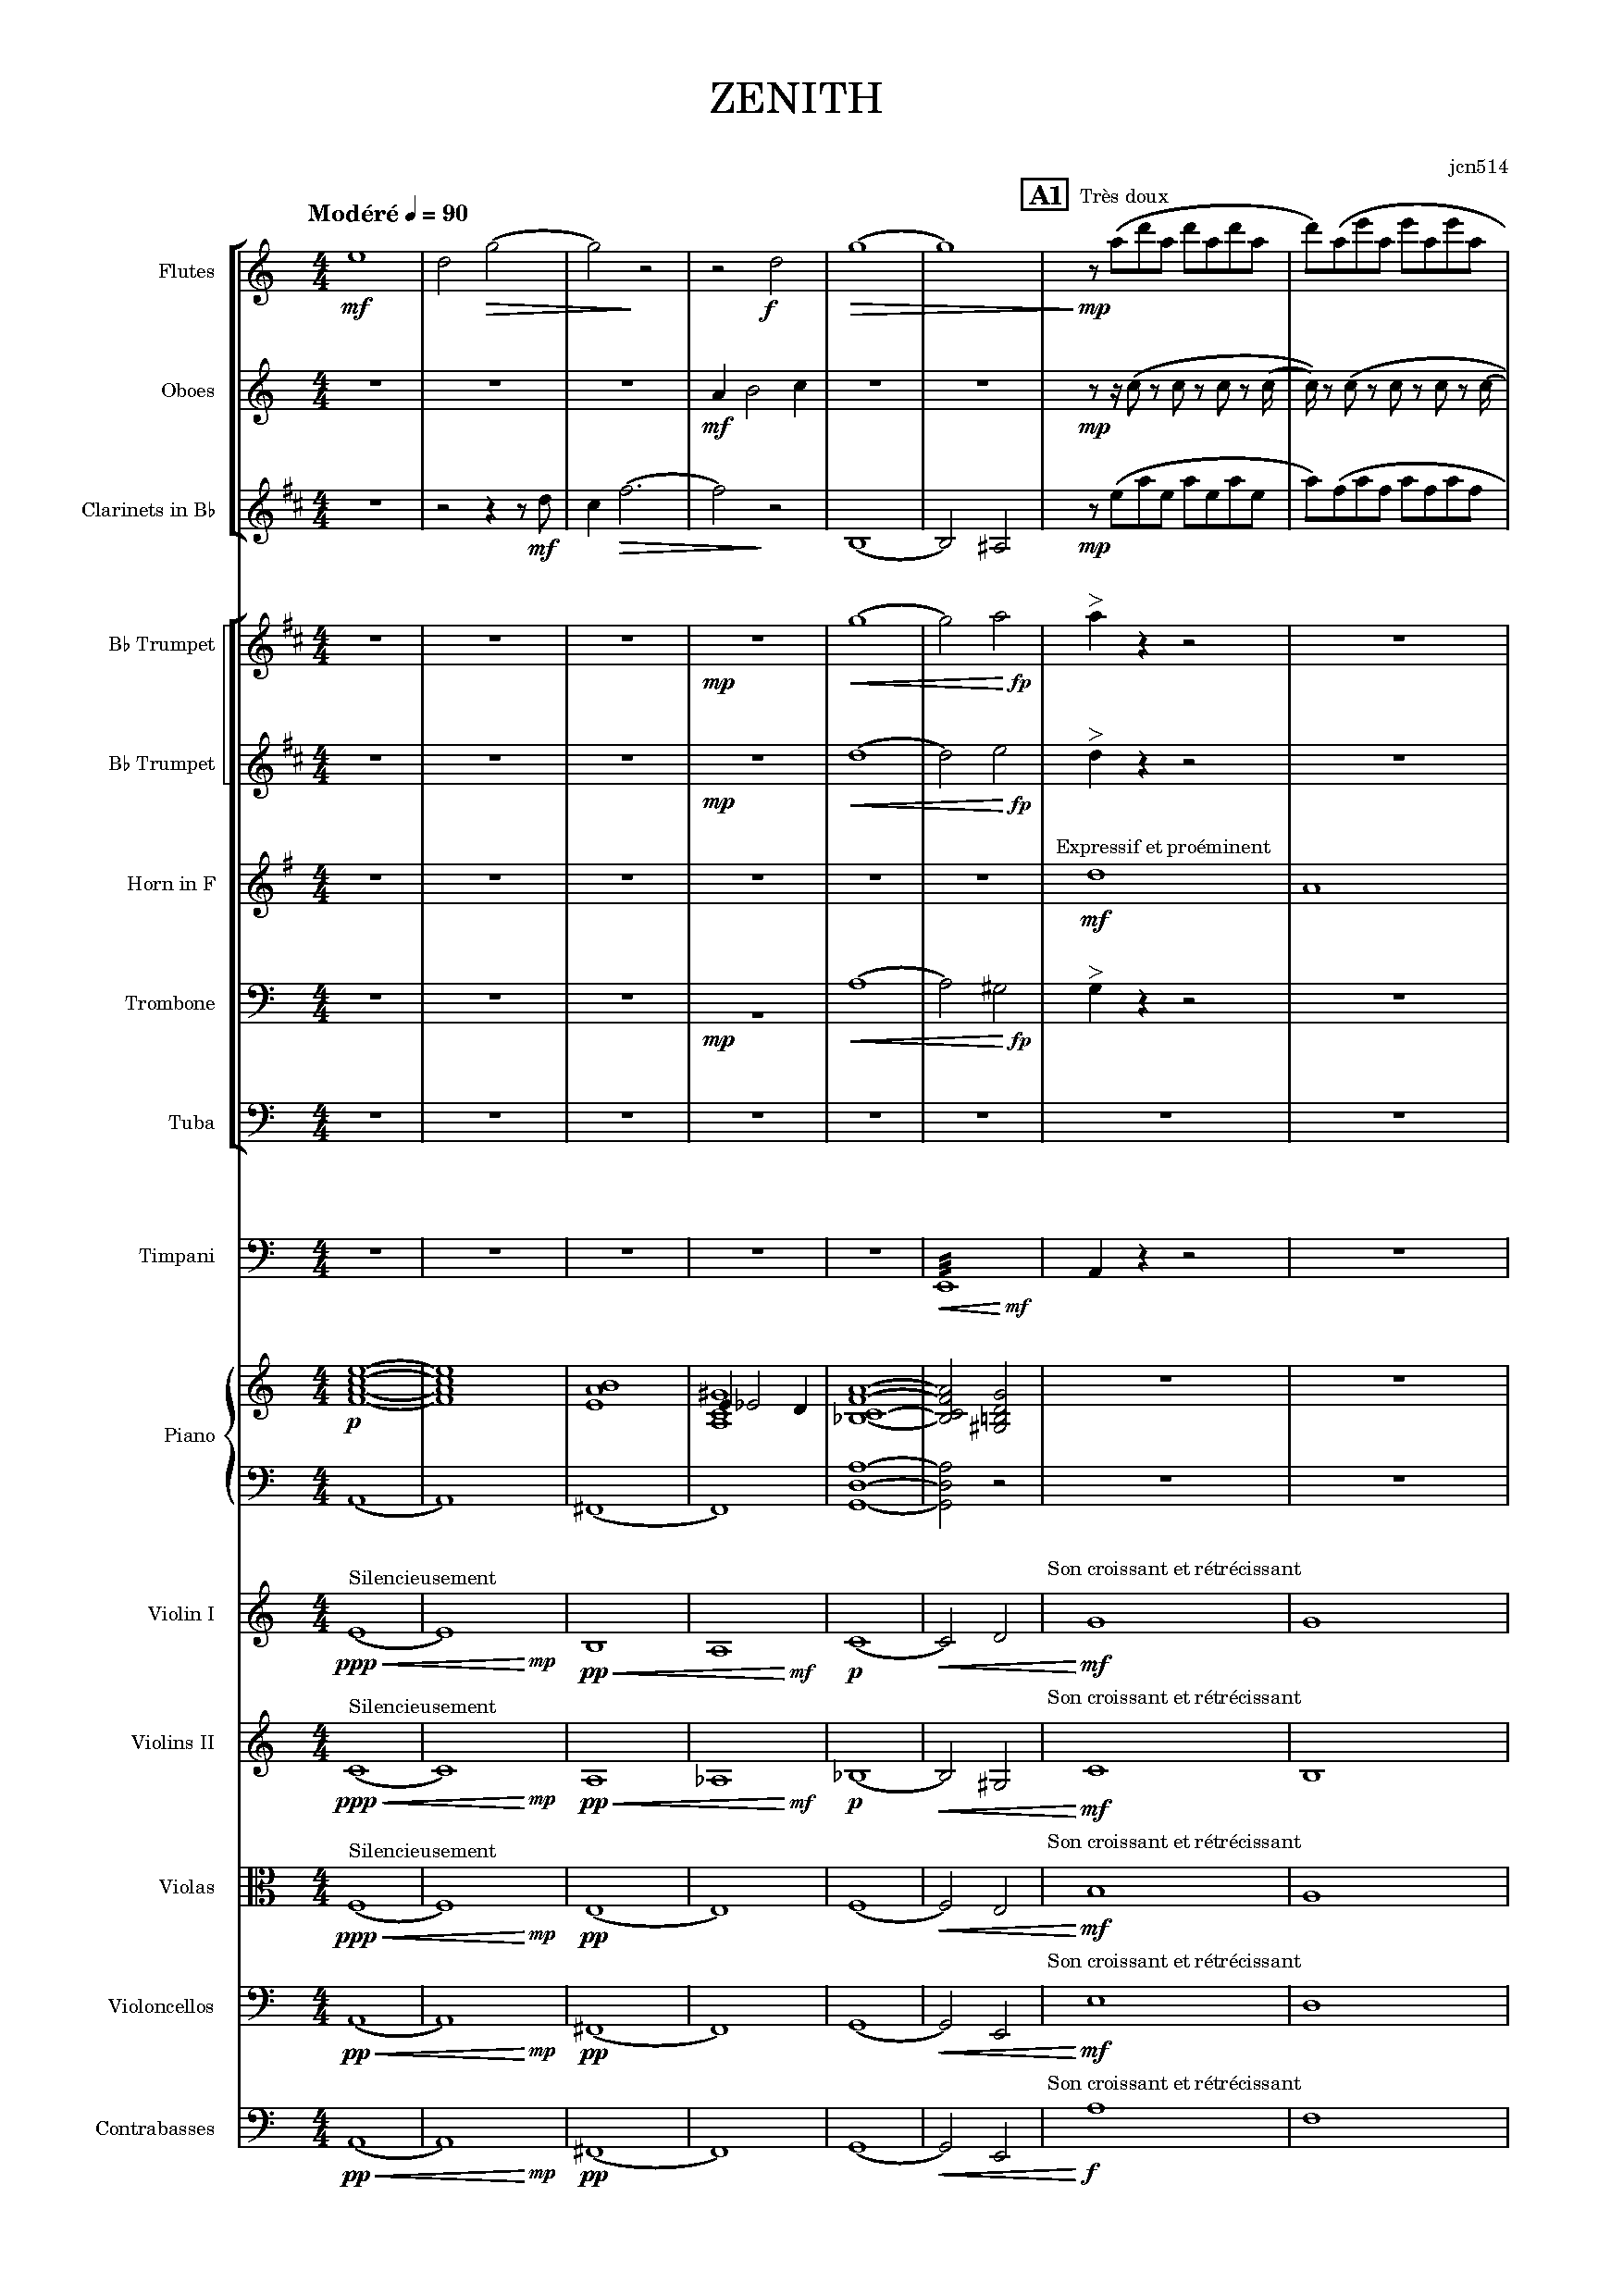
\includepdf[pages=-]{orchestral.pdf}
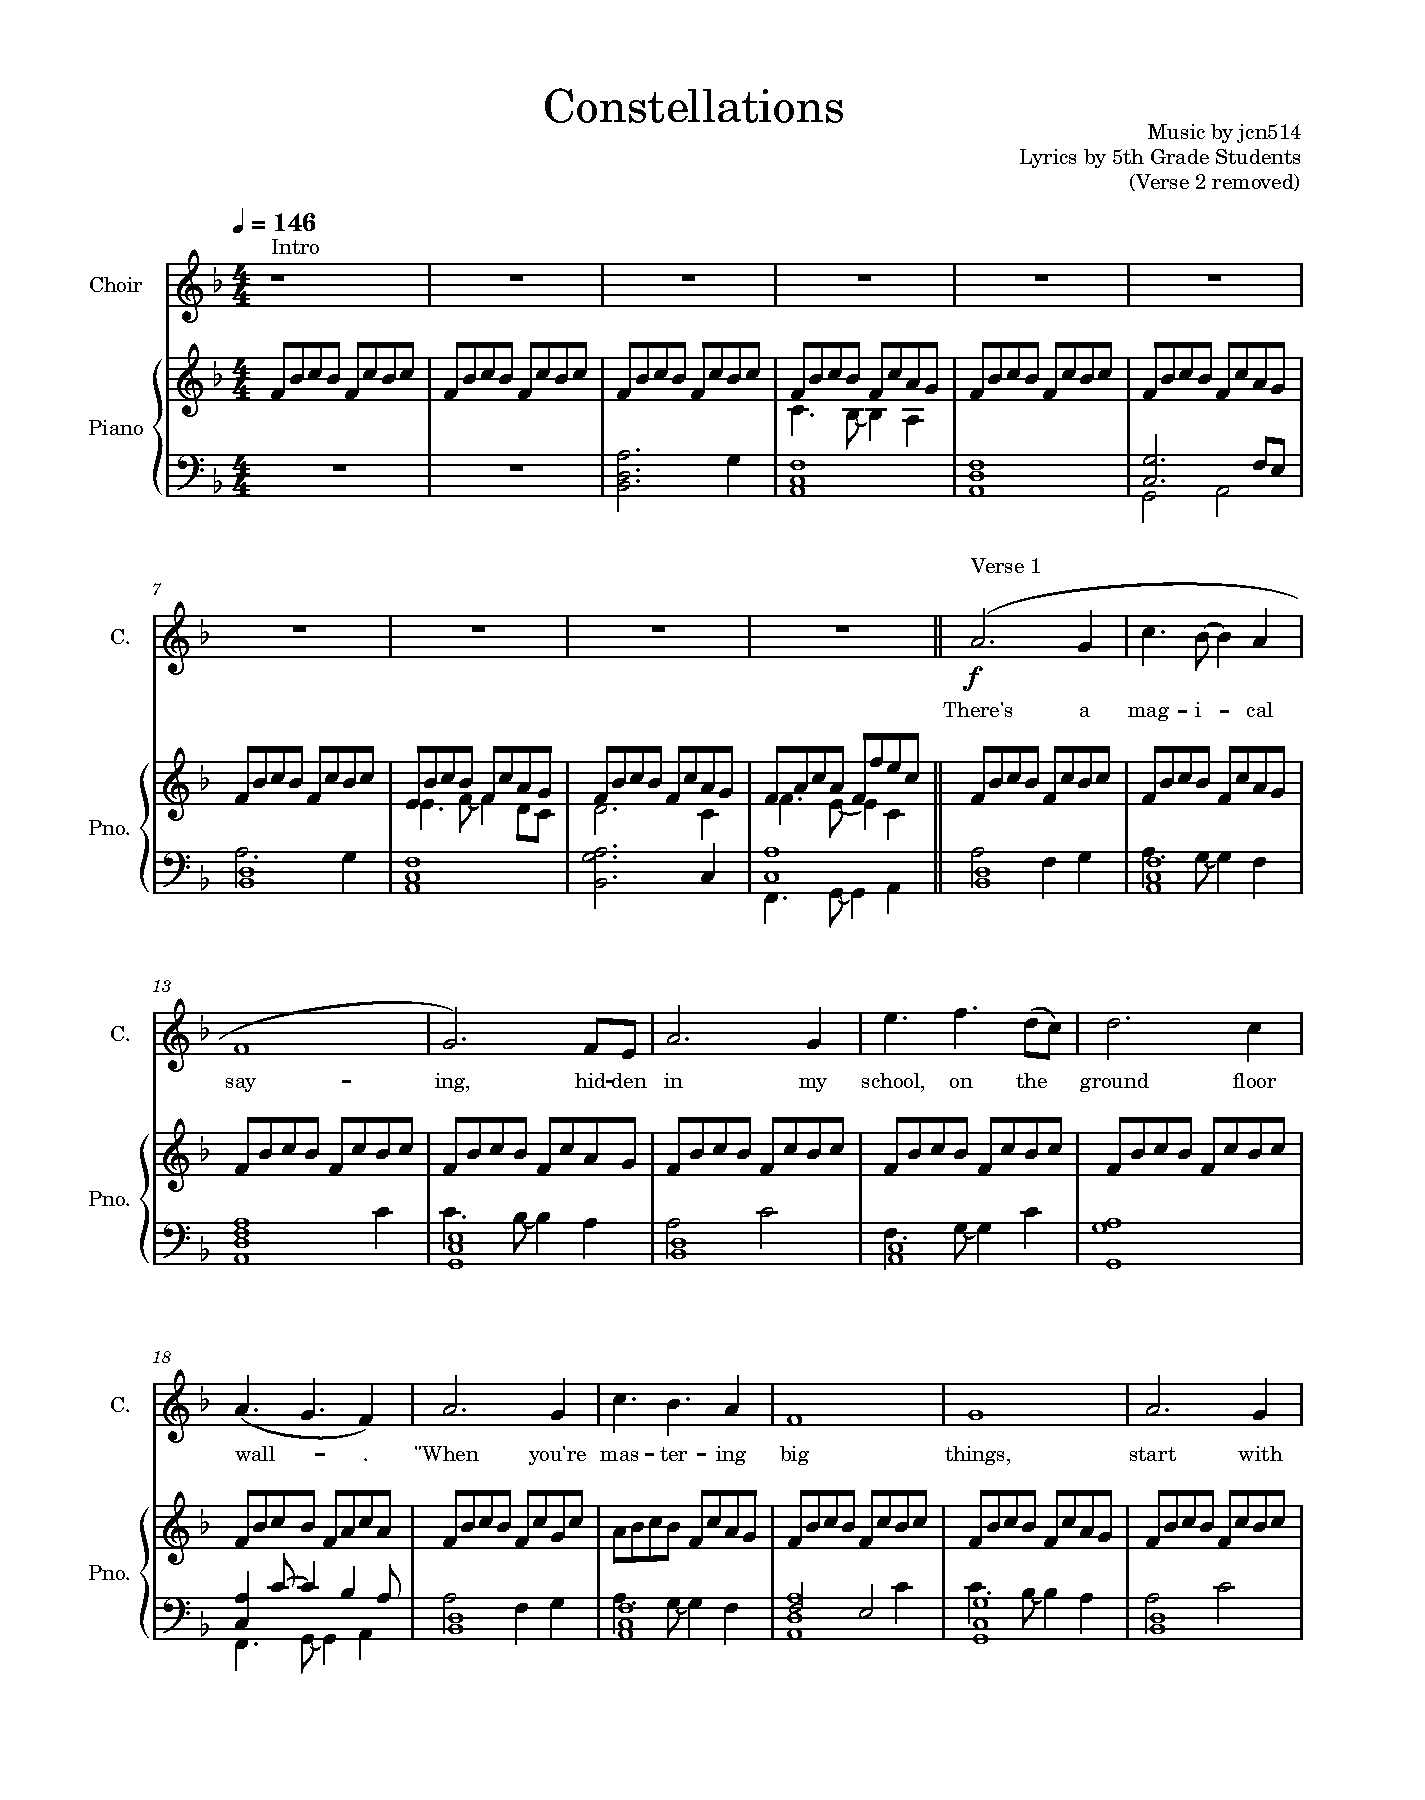
\includepdf[pages=-]{choralPiece.pdf}




\end{document}